\section{Question 1: Sieve of Eratosthenes - OpenMP}

In this task we were asked to rewrite our implementation of the \textit{Sieve of Eratosthenes} using OpenMP instead of Posix Threads. 
\begin{itemize}
  \item Step one of this task was to remove any references to posix threads (this included thread creation, locks and joins). 
  \item Step two was then to implement OpenMP by using specific OpenMP constructs such as:
  \begin{itemize}
    \item \#pragma omp parallel num\_threads(numThreads) - with the number of requested threads as a command line argument 
    \item \#pragma omp single - to run the serial initiation of the seeds 
    \item \#pragma omp for - to split up the workload between the threads in an as even fashion as possible
  \end{itemize}
  \item Step three was to compile and test the code, and finally compare results 
\end{itemize}
Note that one could have set the number of requested threads using the environment variable \textit{OMP\_NUM\_THREADS}, 
however to stay true to the implementation of the original code it was decided to set it explicitly using a command-line argument.

For the complete implementation please see the attached code file \textit{sieve.cpp}

The OpenMP implementation was far easier to write when compared to the Posix version. 
Many functions were able to be dropped and the code became far more readable and concise.
The code is also far safer as it is easier to understand. And the written implementation allows it to be run on a single-threaded system without any code changes. 

\subsection{Results}
All results are from the \textit{vitsippa.it.uu.se} system.

As per previous tests, we can see that for small max numbers (10 or 100), the overhead of threads actually increases the amount of time taken to compute the results.
This is shown in figure \ref{fig:sieve10100}. However as we hit medium max numbers (1000000 or 10000000), we already see an approx 50\% reduction of time as we increase number of threads.
This is shown in figure \ref{fig:sieve100000010000000}. 
And as we hit large max numbers we see that we have hit 50\% reduction per addition of threads.
This is shown in figure \ref{fig:sieve90000000}.

\begin{figure}
  \centering
  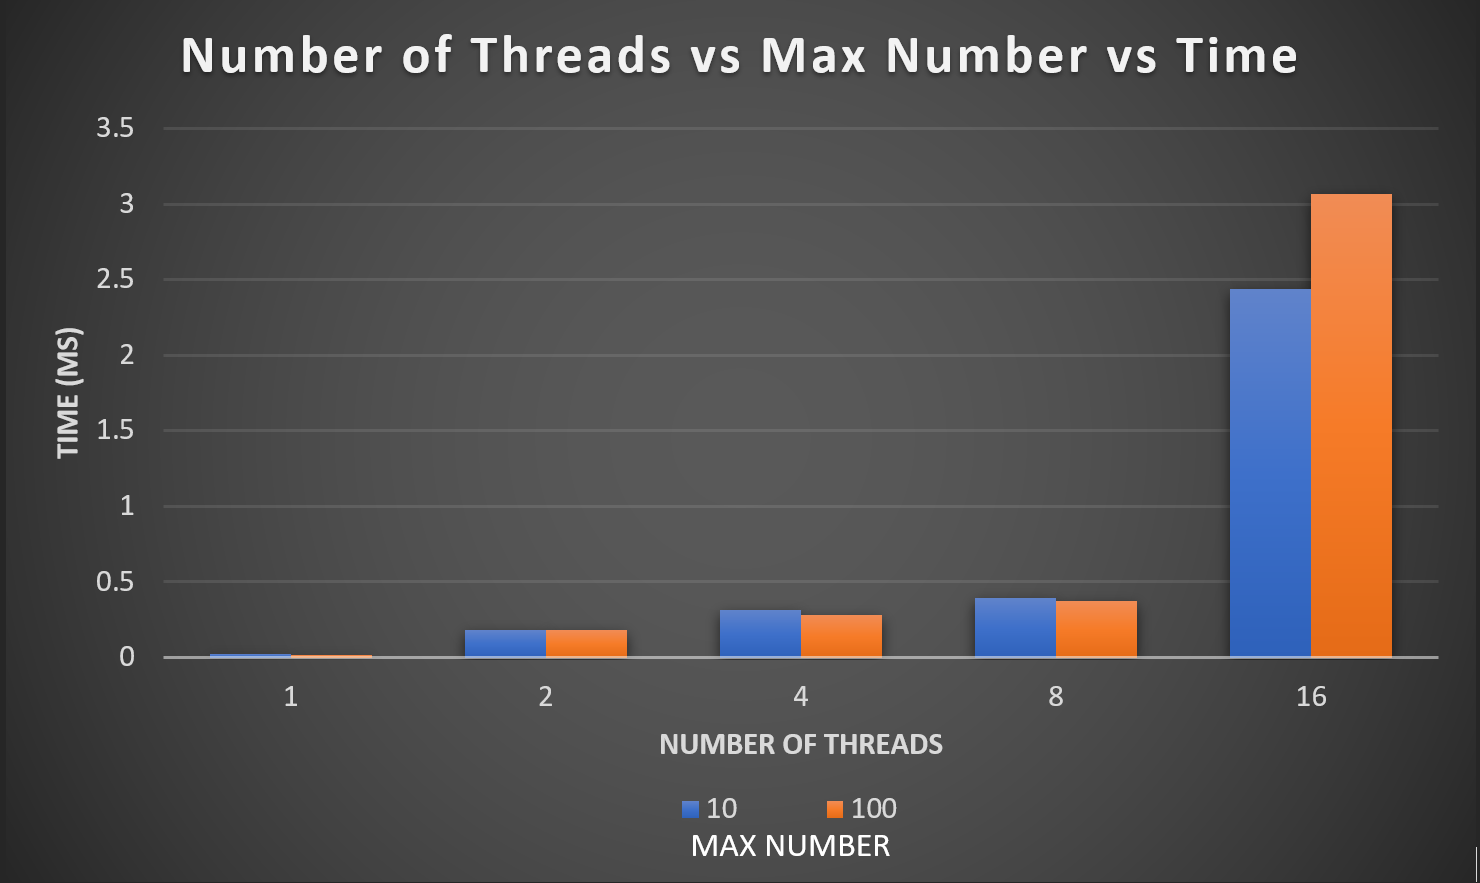
\includegraphics[width=\linewidth]{Figures/results_small.png}
  \caption{Sieve of Eratosthenes with max number $10$ and $100$.}
  \label{fig:sieve10100}
\end{figure}

\begin{figure}
  \centering
  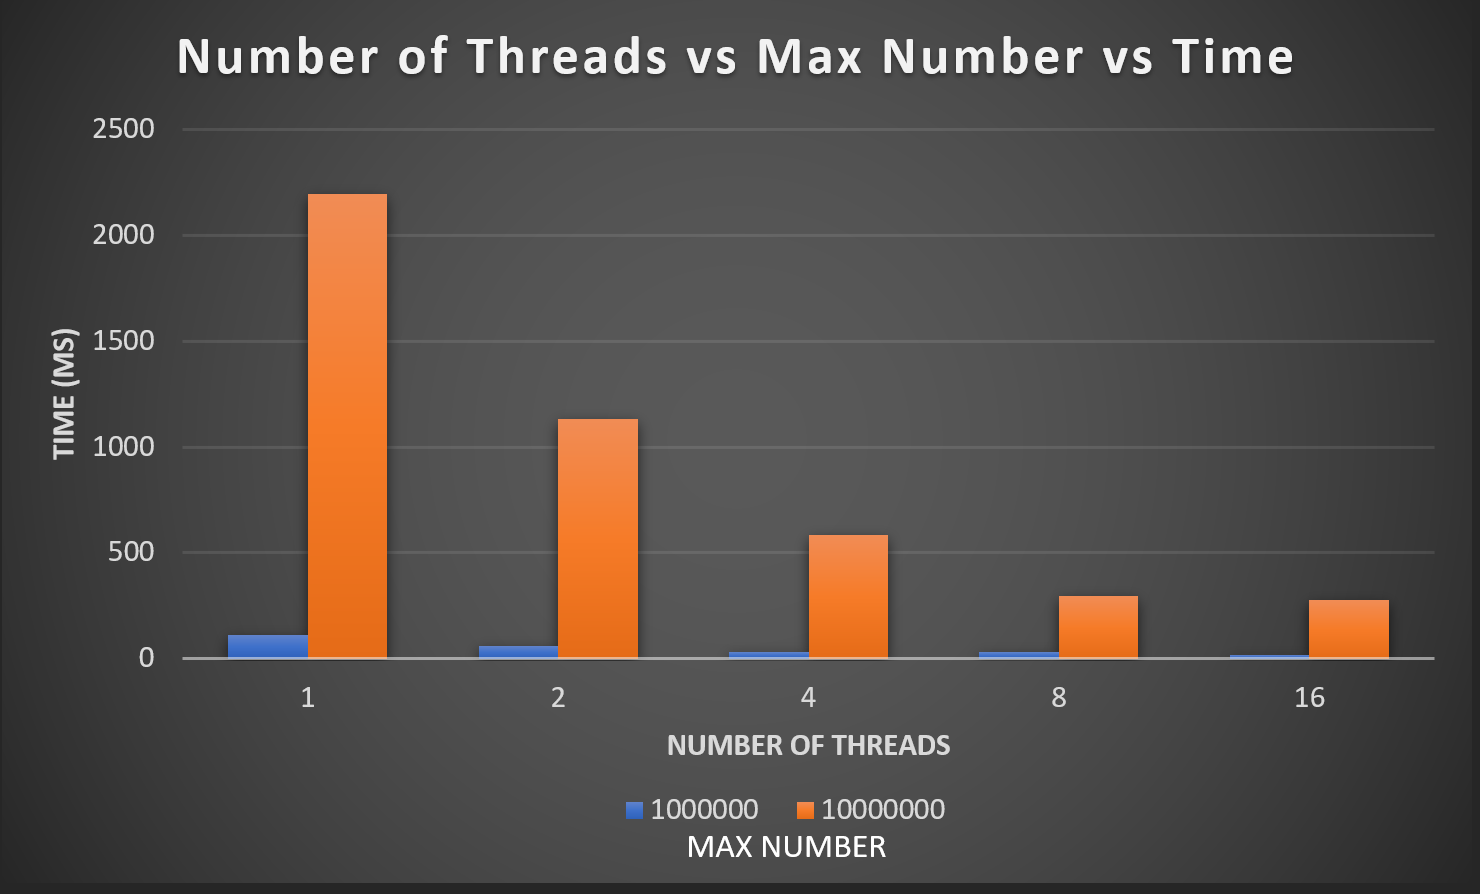
\includegraphics[width=\linewidth]{Figures/results_med.png}
  \caption{Sieve of Eratosthenes with max number $10^6$ and $10^7$.}
  \label{fig:sieve100000010000000}
\end{figure}

\begin{figure}
  \centering
  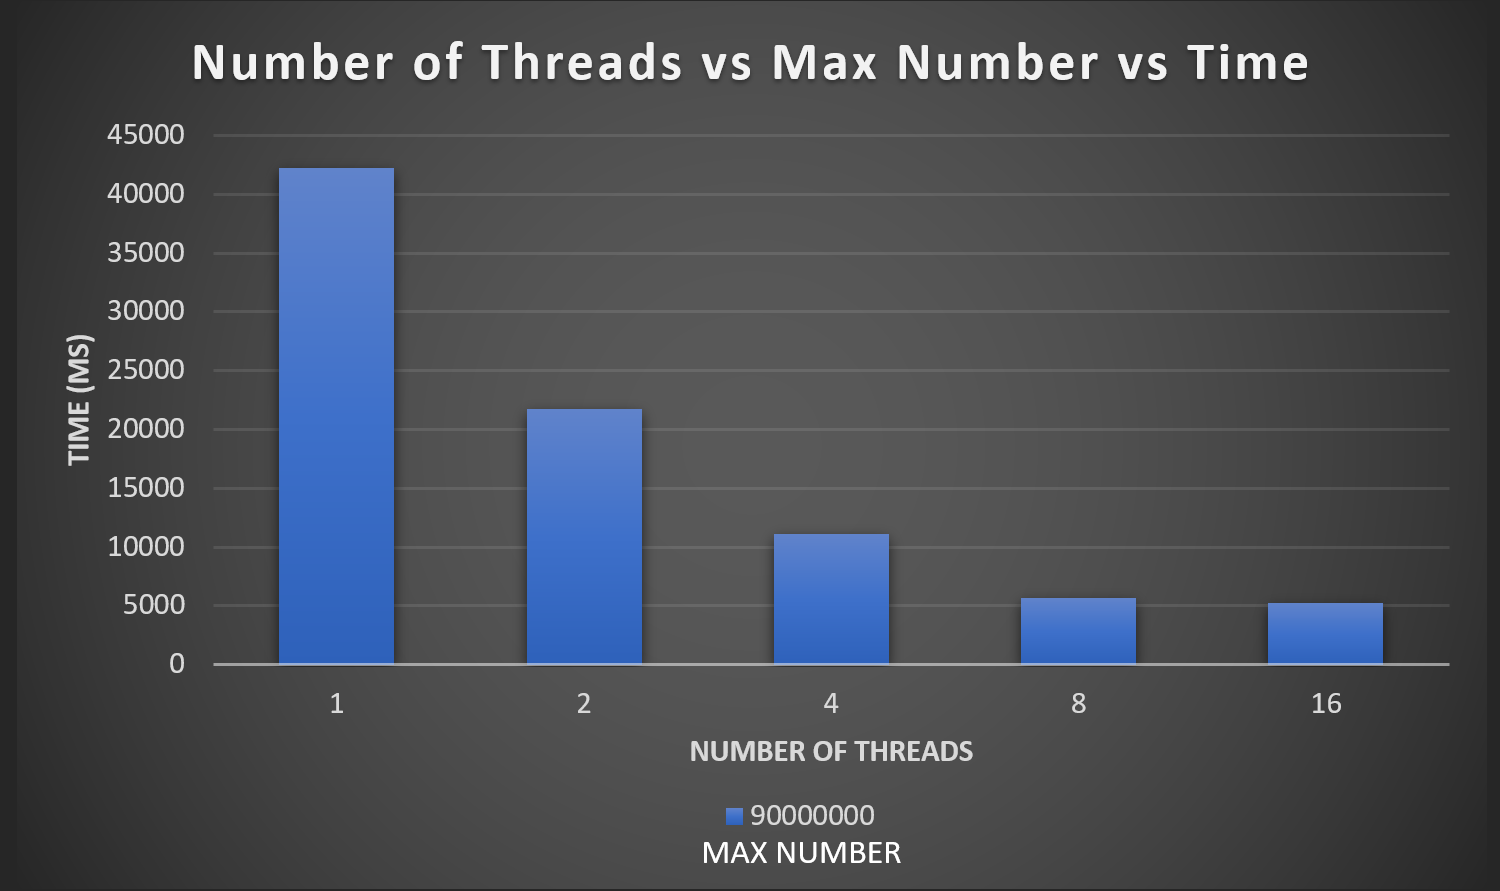
\includegraphics[width=\linewidth]{Figures/results_large.png}
  \caption{Sieve of Eratosthenes with max number $9\times10^7$.}
  \label{fig:sieve90000000}
\end{figure}

This time decrease hits substantially as we break into larger numbers as we overcome the overhead that parallelizing the application adds (and thus can take advantage of the threads)
\textit{Note: the difference between 8 and 16 threads are nominal, this indicates that the system was unable to give us a full 16 threads at testing time, however should we have gotten them, we would expect to see a full 50\% reduction in time}
Interestingly if we compare the runs of the Posix version to the OpenMP, we see a significant reduction in times (almost 75\%). 
This is likely due to the less overhead OpenMP adds to parallelize the application vs our implementation Posix threads (with the additional functions and jumps).
See figure \ref{fig:sievePosixVsOpenMp}.

\begin{figure}
  \centering
  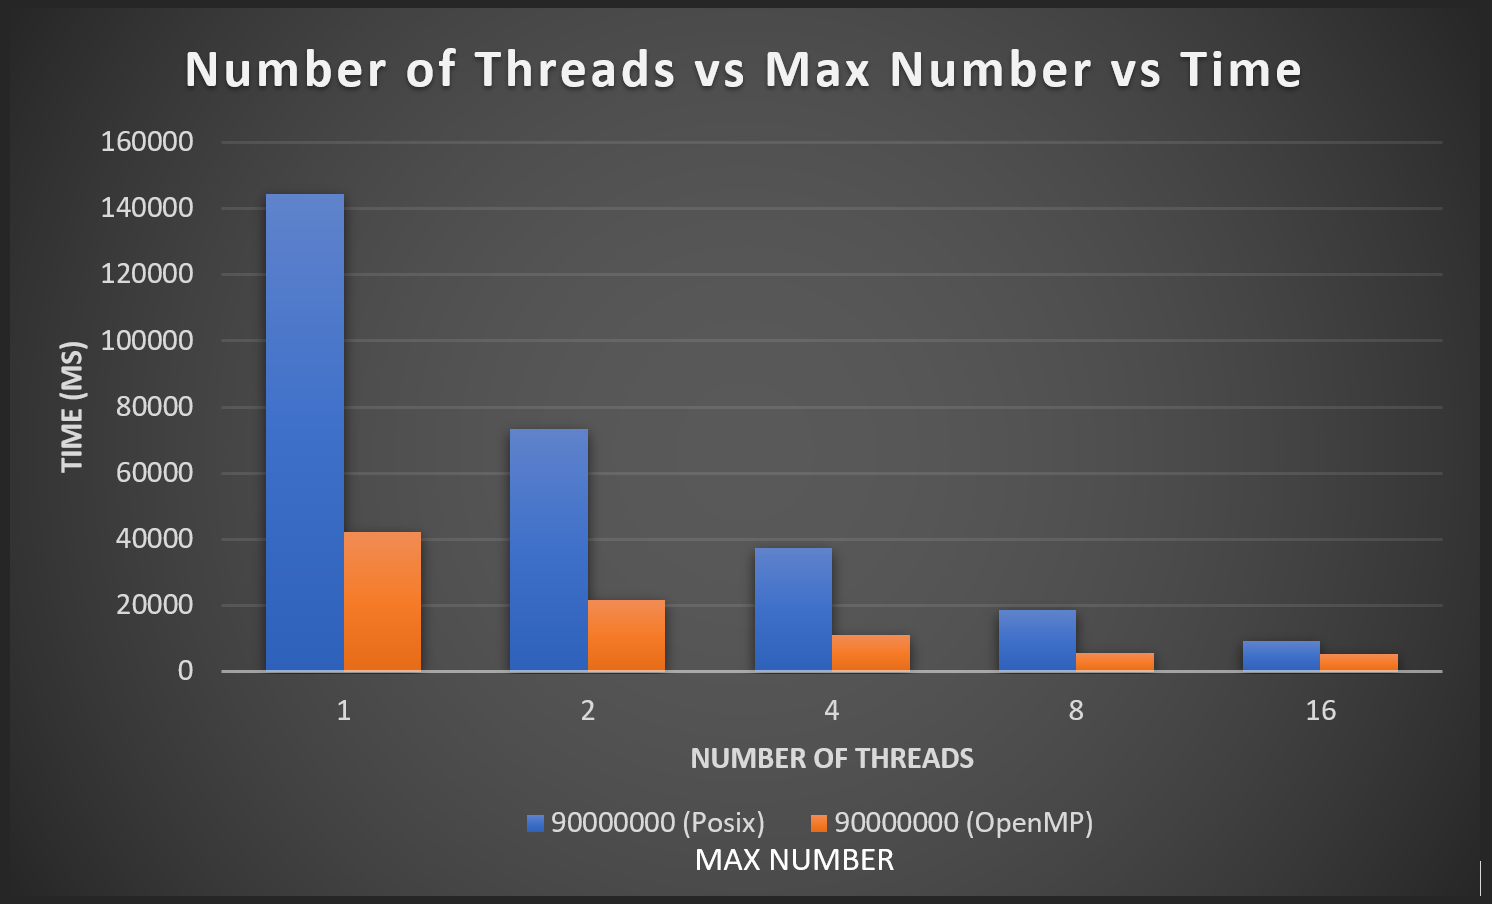
\includegraphics[width=\linewidth]{Figures/posixVsOpenMP.png}
  \caption{Posix Threads vs OpenMP.}
  \label{fig:sievePosixVsOpenMp}
\end{figure}